\documentclass[english,11pt]{beamer}

\DeclareMathOperator{\Cov}{Cov}
\DeclareMathOperator{\Var}{Var}
\DeclareMathOperator{\E}{\mathbb{E}}
\DeclareMathOperator{\Proba}{\mathbb{P}}

\newcommand{\Covb}[2]{\ensuremath{\Cov\!\left[#1,#2\right]}}
\newcommand{\Eb}[1]{\ensuremath{\E\!\left[#1\right]}}
\newcommand{\Pb}[1]{\ensuremath{\Proba\!\left[#1\right]}}
\newcommand{\Varb}[1]{\ensuremath{\Var\!\left[#1\right]}}

% norm
\newcommand{\norm}[1]{\| #1 \|}

\newcommand{\indep}{\rotatebox[origin=c]{90}{$\models$}}





\usepackage{mathptmx,amsmath,amssymb,graphicx,bibentry,bbm,babel,ragged2e}

\makeatletter

\newcommand{\noun}[1]{\textsc{#1}}
\newcommand{\jitem}[1]{\item \begin{justify} #1 \end{justify} \vfill{}}
\newcommand{\sframe}[2]{\frame{\frametitle{#1} #2}}

\newenvironment{centercolumns}{\begin{columns}[c]}{\end{columns}}
%\newenvironment{jitem}{\begin{justify}\begin{itemize}}{\end{itemize}\end{justify}}

\usetheme{Warsaw}
\setbeamertemplate{footline}[text line]{}
\setbeamertemplate{headline}{}
\setbeamercolor{structure}{fg=purple!50!blue, bg=purple!50!blue}

\setbeamersize{text margin left=15pt,text margin right=15pt}

\setbeamercovered{transparent}


\@ifundefined{showcaptionsetup}{}{%
 \PassOptionsToPackage{caption=false}{subfig}}
\usepackage{subfig}

\usepackage[utf8]{inputenc}
\usepackage[T1]{fontenc}

\usepackage{multirow}


\makeatother




\begin{document}

\title{A meta-analysis of models for interactions between transportation networks and territories}
\author{J.~Raimbault$^{1,2,3\ast}$\\
\texttt{j.raimbault@ucl.ac.uk}
}


\institute{$^{1}$CASA, UCL\\
$^{2}$UPS CNRS 3611 Complex Systems Institute Paris\\
$^{3}$UMR CNRS 8504 G{\'e}ographie-cit{\'e}s
}


\date{ECTQG 2019\\
Co-evolution of cities and networks\\
September 7th 2019
}

\frame{\maketitle}


% 
%\textbf{Keywords: }\textit{Network-territories interaction models; Systematic review; Meta-analysis}



\sframe{Interactions between networks and territories}{

% The dynamics of territorial systems have extensively been studied in their interaction with transportation networks which are assumed to play a significant role in their trajectories.

% CN quali slide


\justify

\begin{center}
\includegraphics[width=0.45\linewidth]{figures/accessp_withbridge_prd_EN.png}
\hspace{0.1cm}
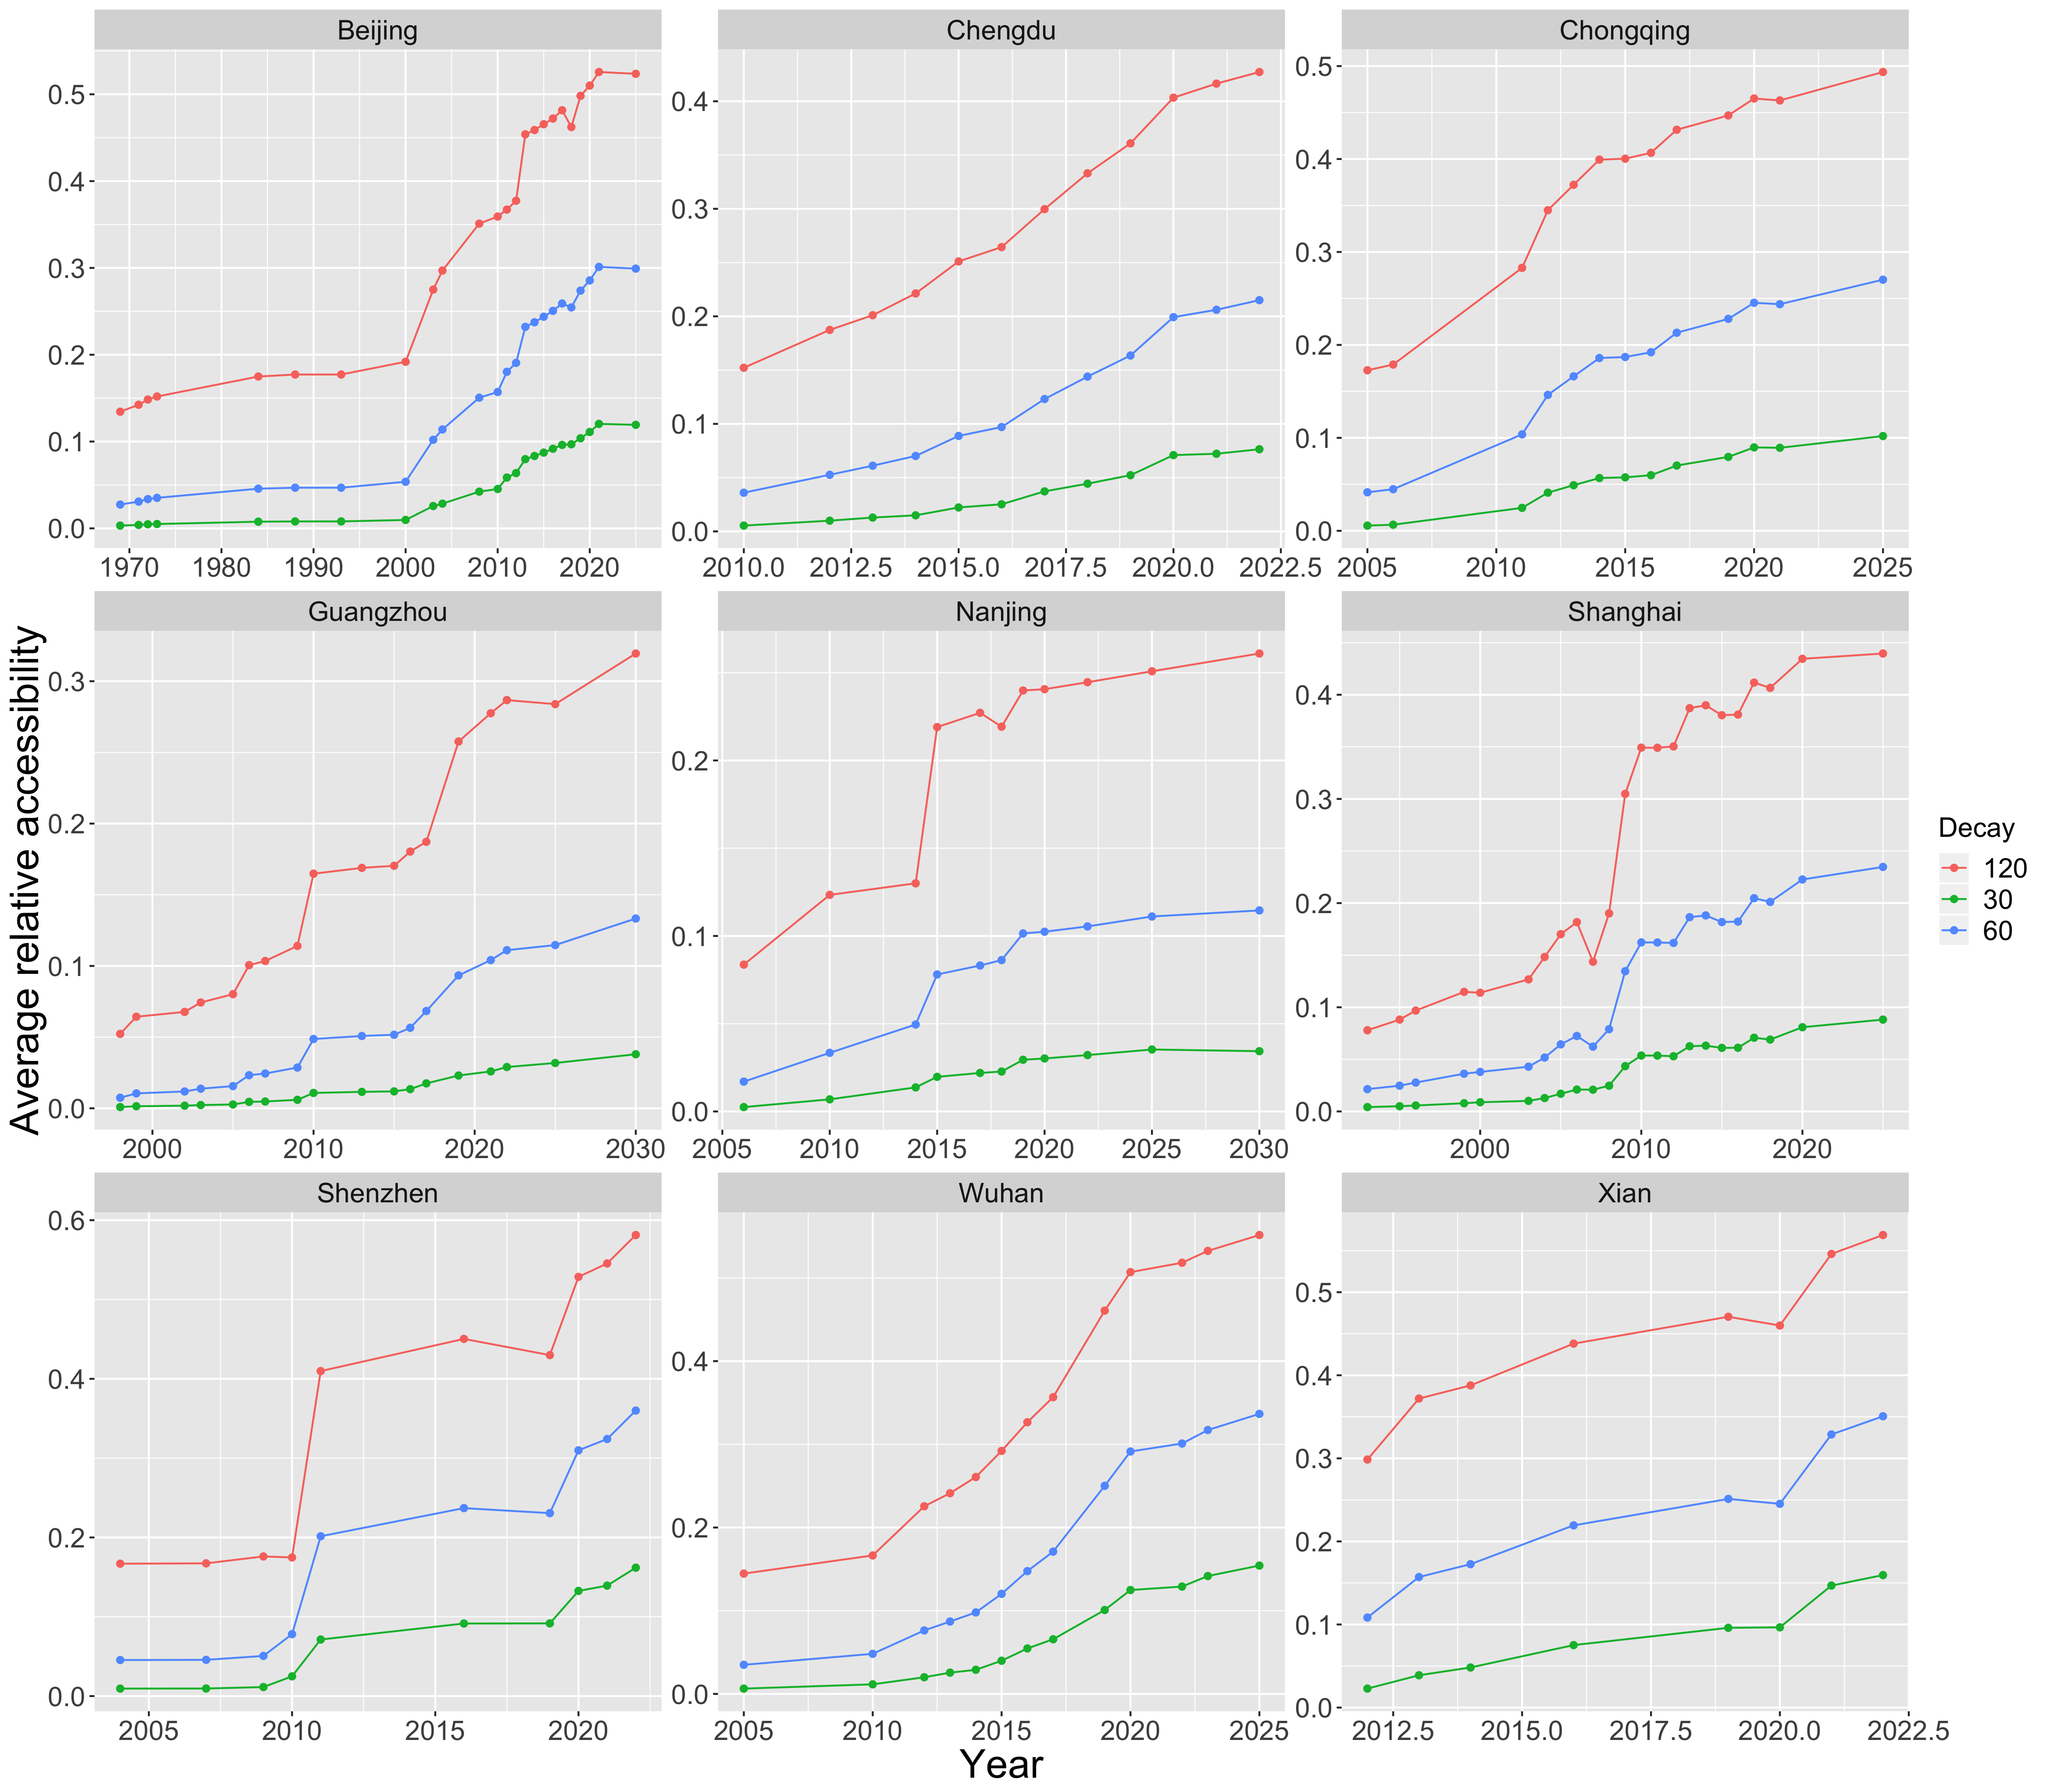
\includegraphics[width=0.52\linewidth]{figures/avgaccess_facet.png}

\end{center}

\medskip

%\vspace{-0.5cm}

%\begin{justify}
\textit{Accessibility as part of complex processes of co-evolution between transportation networks and territories.}

%\end{justify}

\nocite{raimbault:halshs-02265423}

\medskip

\tiny

Raimbault, J. (2019). Evolving accessibility landscapes: mutations of transportation networks in China. In Aveline-Dubach, N., ed. \textit{Pathways of sustainable urban development across China - the cases of Hangzhou, Datong and Zhuhai}, pp 89-108. Imago. ISBN:978-88-94384-71-0

}



\sframe{Interaction processes}{

% processes from the lit review / chap 1 ?

\textit{Stylized interaction processes between transportation networks and territories}

\medskip

\begin{center}
\begin{tabular}{|c|p{2.8cm}|p{2.8cm}|p{2.8cm}|}
\hline
 & Networks $\rightarrow$ Territories & Territories $\rightarrow$ Networks & Networks $\leftrightarrow$ Territories\\ \hline
Micro & Mobility patterns & Network congestion ; Negative externalities & Mobility and social structure \\ \hline
Meso & Relocations ; Local effects of infrastructures & Potential breakdown & Metropolitan planning ; TOD \\ \hline
Macro & Interactions between cities ; Tunnel effect & Hierarchical differentiation of accessibility & Large scale planning ; Structural dynamics ; Bifurcations\\ \hline
\end{tabular}
\end{center}

% no need to cite the thesis - results come from it otherwise mentioned
%\nocite{}


}


\sframe{Diverse modeling approaches}{

% Therefore, several modeling approaches focusing on the interactions between transportation networks and territories have been introduced by various disciplines, including for example land-use transport interaction models from planning and transportation science, spatial interaction models or co-evolution models from geography, network growth models from physics.

% -> cit nw analysis ectqg 2017

\textit{Complementary modeling approaches}

\medskip

\begin{center}
	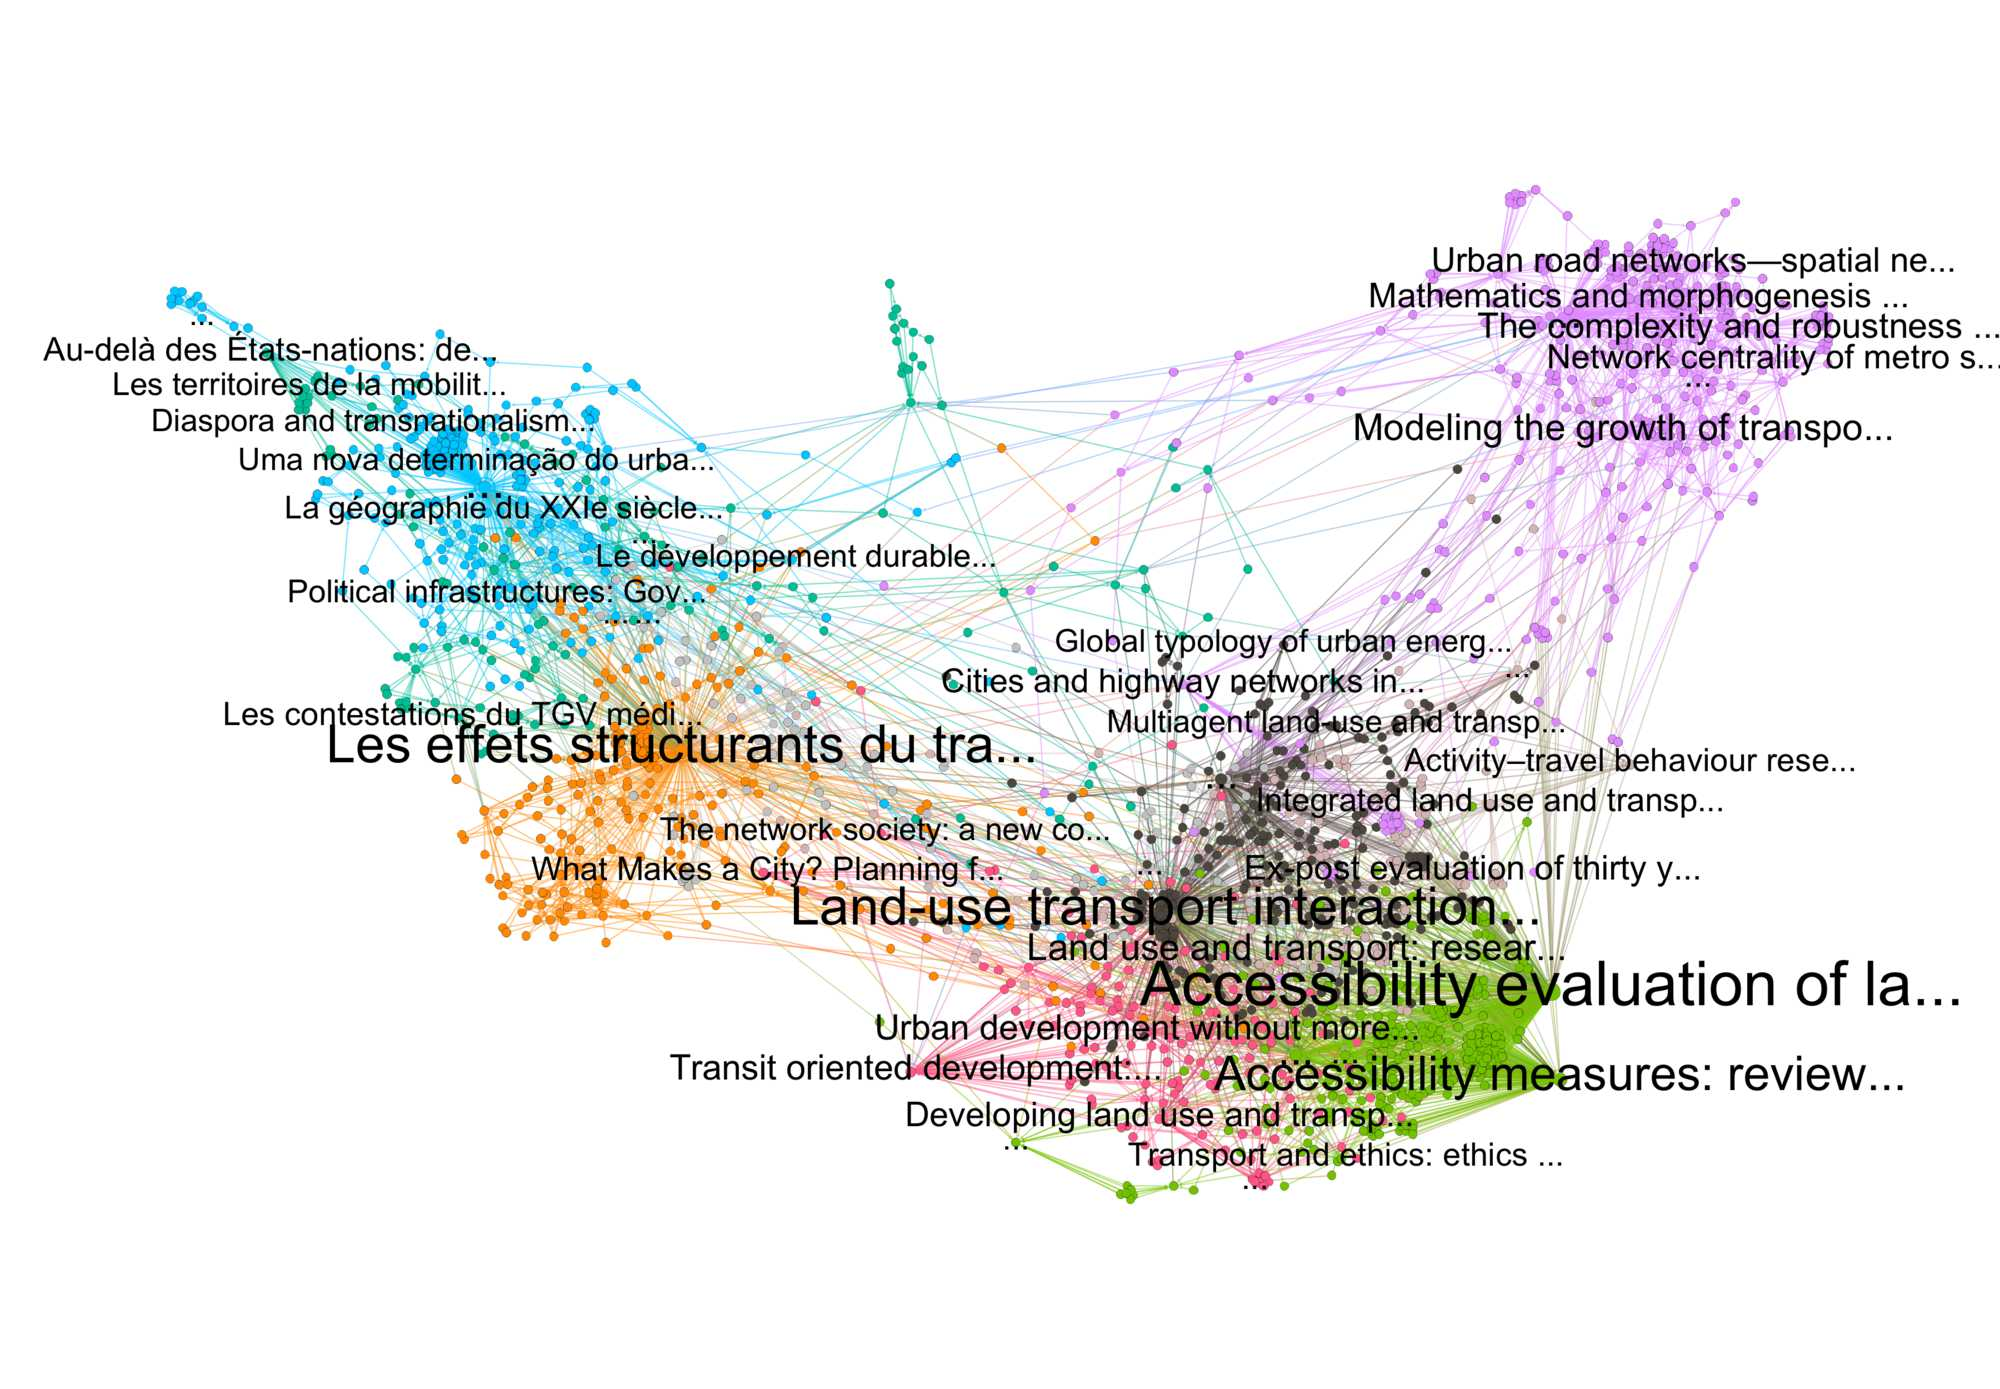
\includegraphics[width=0.9\textwidth,trim={0 2cm 0 2cm},clip]{figures/2-2-2-fig-quantepistemo-citnw.jpg}	
\end{center}

\medskip

\tiny

\vspace{-1cm}

Raimbault, J. (2019). Exploration of an interdisciplinary scientific landscape. Scientometrics, 119(2), 617-641.

\nocite{raimbault2019exploration}

}


\sframe{Towards a modelography}{

%  This contribution introduces a systematic review and meta-analysis to understand the nature and properties of these models in relation to their disciplinary context.

% research question

\justify

$\rightarrow$ beyond mapping of the literature, what are typical patterns of models characteristics depending on disciplines?

\medskip

$\rightarrow$ systematic reviews and meta-analysis widely used in STEM \cite{rucker2012network}, less in social sciences and humanities (in geography see \cite{cottineau2017metazipf}, \cite{schmitt2013modelographie})



\bigskip

\textbf{Research objective: }

\medskip

\textit{Construct a corpus of models of interaction between transportation networks and territories, with comparable characteristics; study determinants of these.}


}


\sframe{Corpus construction method}{

%We construct a corpus of models through a systematic review. The raw corpus after initial keyword requests is composed by around 3800 papers, which were screened for inclusion first on their titles (297 papers kept), then on their full-text content resulting in a study corpus of 145 papers.

\begin{enumerate}
	\item Extract most relevant keywords from the previous citation network-semantic scientific mapping (see \cite{raimbault2019exploration} and \cite{raimbault2017invisible})
	\item For each keyword, get a fixed number $n=20$ of references from a catalog request
	\item Merge the corresponding corpus with the references from the citation network
	\item Manual screening on titles, abstracts and full texts if necessary ($N_f = 145$)
\end{enumerate}


}

\sframe{Corpus construction method}{

\centering

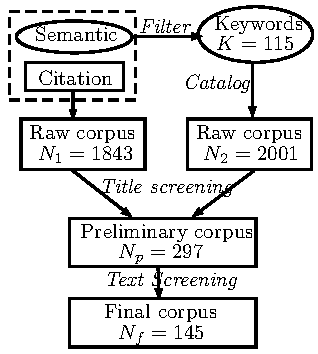
\includegraphics[height=0.9\textheight]{figures/systematicreview.pdf}

}

\sframe{Systematic review}{

Lessons from the systematic review:

\medskip

\begin{itemize}
\item Catalog bias seem unavoidable
\item Availability of full texts is a crucial point (\url{http://sci-hub.tw/} saved the study)
\item Journals and editors increase visibility and request bias, grey literature has different status depending on the field
\item Manual screening is also useful to discover important papers that can be missed in classical review
\item Systematic review results are significantly different from the subjective manual review (both are complementary)
\end{itemize}


}

% thematic observations - not useful
% \item The articles selected imply a clarification of what is meant by ``model''. We give in~\ref{sec:knowledgeframework} a very broad definition applying to all scientific perspectives. Our selection here does not retain conceptual models for example, our choice criteria being that the model must include a numerical or simulation aspect.
%	\item A certain number of references consist in reviews, what is equivalent to a group of model with similar characteristics. % TODO this is not necessarily true, a review can compare very different ways to study the same object e.g.
%	We could make the method more complicated by transcribing each review or meta-analysis, or by weighting the records of corresponding characteristics by the corresponding number of articles. We make the choice to ignore these reviews, what remains consistent in a thematic way still with the assumption of uniform sampling.
%	\item A first clarification of the thematic frame is achieved, since we do not select studies uniquely linked to traffic and mobility (this choice being also linked to the results obtained in~\ref{sec:transportationequilibrium}), to pure urban design, to pedestrian flows models, to logistics, to ecology, to technical aspects of transportation, to give a few examples, even if these subjects can in an extreme view be considered as linked to interactions between networks and territories.
%	\item Similarly, neighbor fields such as tourism, social aspects of the access to transportation, anthropology, were not taken into account.
%	\item We observe a high frequency of studies linked to High Speed Rail (HSR), recalling the necessary association of political aspects of planning and of research directions in transportation.




\sframe{Extracted characteristics}{

%For each model, properties are extracted including the type of coupling (weak or strong and the direction) between network and territory, spatial and temporal scales, the methodology used, and the discipline, in order to proceed to a meta-analysis of these.

For each model we extract:

\medskip

\begin{itemize}
	\item strength of coupling among: \texttt{\{territory ; network ; weak ; coevolution\}}
	\item maximal time scale
	\item maximal spatial scale
	\item domain ``a priori'' (domain of journal)
	\item methodology used %(statistical models, system of equations, multi-agent, cellular automaton, operational research, simulation, etc.)
	\item case study when relevant % (city, metropolitan area, region or country)
	\item thematic question and processes %(\textit{too broad, not used})
\end{itemize}

\medskip

From multilayer scientific landscaping (semantic classification recomputed for this corpus) we obtain:

\begin{itemize}
	\item citation domain
	\item semantic domain
	\item index of interdisciplinarity
\end{itemize}


}

\sframe{Strength of model coupling}{

\centering

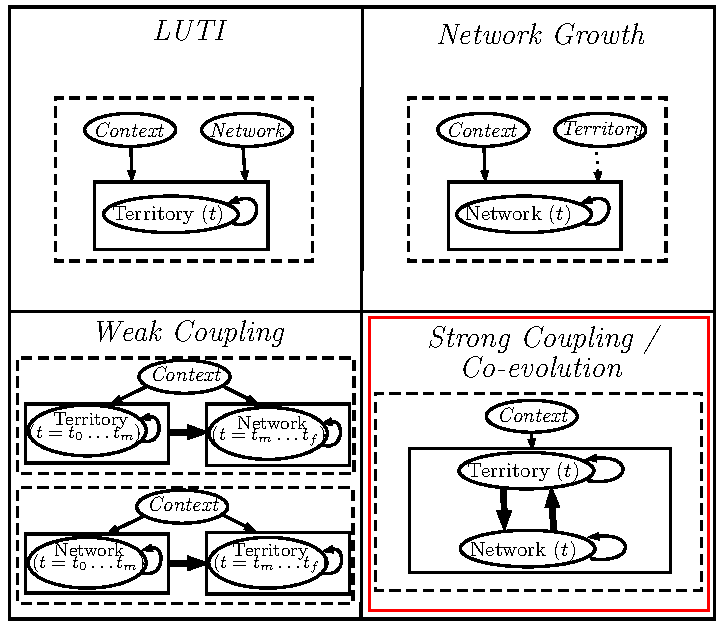
\includegraphics[width=0.85\textwidth]{figures/coevolution.pdf}

}


\sframe{Exploratory analysis}{

%Exploratory analysis confirms the diversity of approaches existing, 

Descriptive analysis:

\medskip

\begin{itemize}
	\item 26\% with no case study
	\item overrepresentation of Netherlands (6.9\%)
	\item majority of accessibility studies (65\% of studies)
	\item very diverse processes and domains
	\item macroscopic geographical studies are in minority
\end{itemize}

\bigskip

\textbf{Disciplines: } 17.9\% Transportation, 20.0\% Planning, 30.3\% Economics, 19.3\% Geography, 8.3\% Physics

\medskip

\textbf{Semantic domains: } TOD (27.6\%), networks (20.7\%), hedonic models (11.0\%), infrastructure planning (5.5\%), HSR (2.8\%)

}


\sframe{Models characteristics}{

\centering
\small

\begin{tabular}{|c|ccccc|}
\hline
Discipline  &  economics & geography & physics & planning & transportation\\\hline
network     &     5      &      3    &   12    &    1     &         4  \\
strong      &     4      &     3     &   0     &   0      &        2  \\
territory   &    35      &    22     &   0     &    28    &         20 \\\hline  
\end{tabular} 
\medskip
\begin{tabular}{|c|cccccc|}
\hline
Citation  &  accessibility & geography & infra planning & LUTI & networks & TOD \\\hline
network   &            0   &     0     &         0      &   0  &     24   &  0 \\
strong    &            0   &      0    &          0     &   2  &      5   &  0 \\
territory &           13   &      1    &          6     &  18  &      2   &  3 \\\hline
\end{tabular}
\medskip
\begin{tabular}{|c|ccccc|}
\hline
Semantic  &  hedonic & hsr & infra planning & networks & tod\\\hline
network   &       1  & 0   &          0     &  14      & 2 \\
strong    &       0  &  0  &            0   &     5    & 1  \\
territory &      15  &  4  &            8   &    11    &  37 \\ \hline
\end{tabular}

\bigskip

+ Methods and spatial scale significantly correlated with discipline


}


\sframe{Statistical analysis}{

%whereas statistical analysis links type of models and disciplines with properties, showing for example the strong influence of the type of coupling with time scale, or of the discipline on the spatial scale.

%
%\begin{tabular}{lcccccc} 
%\tiny
%\\[-1.8ex]\hline 
%\hline \\[-1.8ex] 
% & \multicolumn{6}{c}{\textit{Explained variable:}} \\ 
%\cline{2-7} 
% & \multicolumn{2}{c}{TEMPSCALE} & SPATSCALE & \multicolumn{2}{c}{INTERDISC} & YEAR \\ 
% & (1) & (2) & (3) & (4) & (5) & (6)\\ 
%\hline \\[-1.8ex] 
% YEAR & 0.674 &  &  & $-$0.004$^{*}$ & $-$0.002$^{*}$ &  \\ 
%  TYPEstrong &  & 100.271$^{***}$ &  &  & $-$0.026 &  \\ 
%  TYPEterritory & $-$38.933$^{***}$ & $-$14.988 &  &  & 0.044 & 10.898$^{***}$ \\ 
%  TEMPSCALE &  &  & $-$5.179 & $-$0.0003 &  & 0.035 \\ 
%  FMETHODeq &  &  &  &  &  & $-$6.224 \\ 
%  FMETHODmap &  &  &  &  &  & 4.747 \\ 
%  FMETHODro &  &  &  &  &  & 6.128 \\ 
%  FMETHODsem &  &  &  &  &  & 1.009 \\ 
%  FMETHODsim &  &  &  &  &  & 5.153 \\ 
%  FMETHODstat &  &  &  &  &  & $-$0.357 \\ 
%  DISCIPLINEengineering & $-$52.107$^{*}$ & $-$9.609 & $-$154.461 & 0.144 &  & 13.486 \\ 
%  DISCIPLINEenvironment & 17.110 & 17.886 & $-$5.878 & 0.092 &  & $-$3.668 \\ 
%  DISCIPLINEgeography & 3.640 & 9.126 & 1,445.457$^{***}$ & 0.036 &  & 1.121 \\ 
%  DISCIPLINEphysics & 46.879$^{*}$ & 77.897$^{***}$ & 292.559 & $-$0.103 &  & 3.392 \\ 
%  DISCIPLINEplanning & 1.304 & 4.553 & $-$143.554 & $-$0.047 &  & $-$2.850 \\ 
%  DISCIPLINEtransportation & $-$14.718 & 8.753 & 568.329 & 0.062 &  & 5.503$^{*}$ \\ 
%  INTERDISC & 2.357 &  &  &  &  & $-$12.876 \\ 
%  SEMCOMcomplex networks &  &  &  &  & $-$0.217 &  \\ 
%  SEMCOMhedonic &  &  &  & $-$0.179 & $-$0.184$^{*}$ & $-$5.769 \\ 
%  SEMCOMhsr &  &  &  & $-$0.100 & $-$0.122 & 6.135 \\ 
%  SEMCOMinfra planning &  &  &  & $-$0.032 & $-$0.096 & $-$4.123 \\ 
%  SEMCOMnetworks &  &  &  & $-$0.038 & $-$0.107 & 4.711 \\ 
%  SEMCOMtod &  &  &  & $-$0.105 & $-$0.152 & $-$1.653 \\ 
%  Constant & $-$1,305.126 & 22.103$^{*}$ & 235.357 & 8.962$^{**}$ & 5.531$^{**}$ & 2,004.945$^{***}$ \\ 
% \hline \\[-1.8ex] 
%Observations & 64 & 94 & 94 & 64 & 98 & 64 \\ 
%R$^{2}$ & 0.385 & 0.393 & 0.100 & 0.314 & 0.155 & 0.510 \\ 
%Adj. R$^{2}$ & 0.282 & 0.336 & 0.027 & 0.136 & 0.068 & 0.281 \\ 
%\hline 
%\hline \\[-1.8ex] 
%\textit{Note:}  & \multicolumn{6}{l}{$^{*}$p$<$0.1; $^{**}$p$<$0.05; $^{***}$p$<$0.01} \\ 
%\end{tabular}


\centering

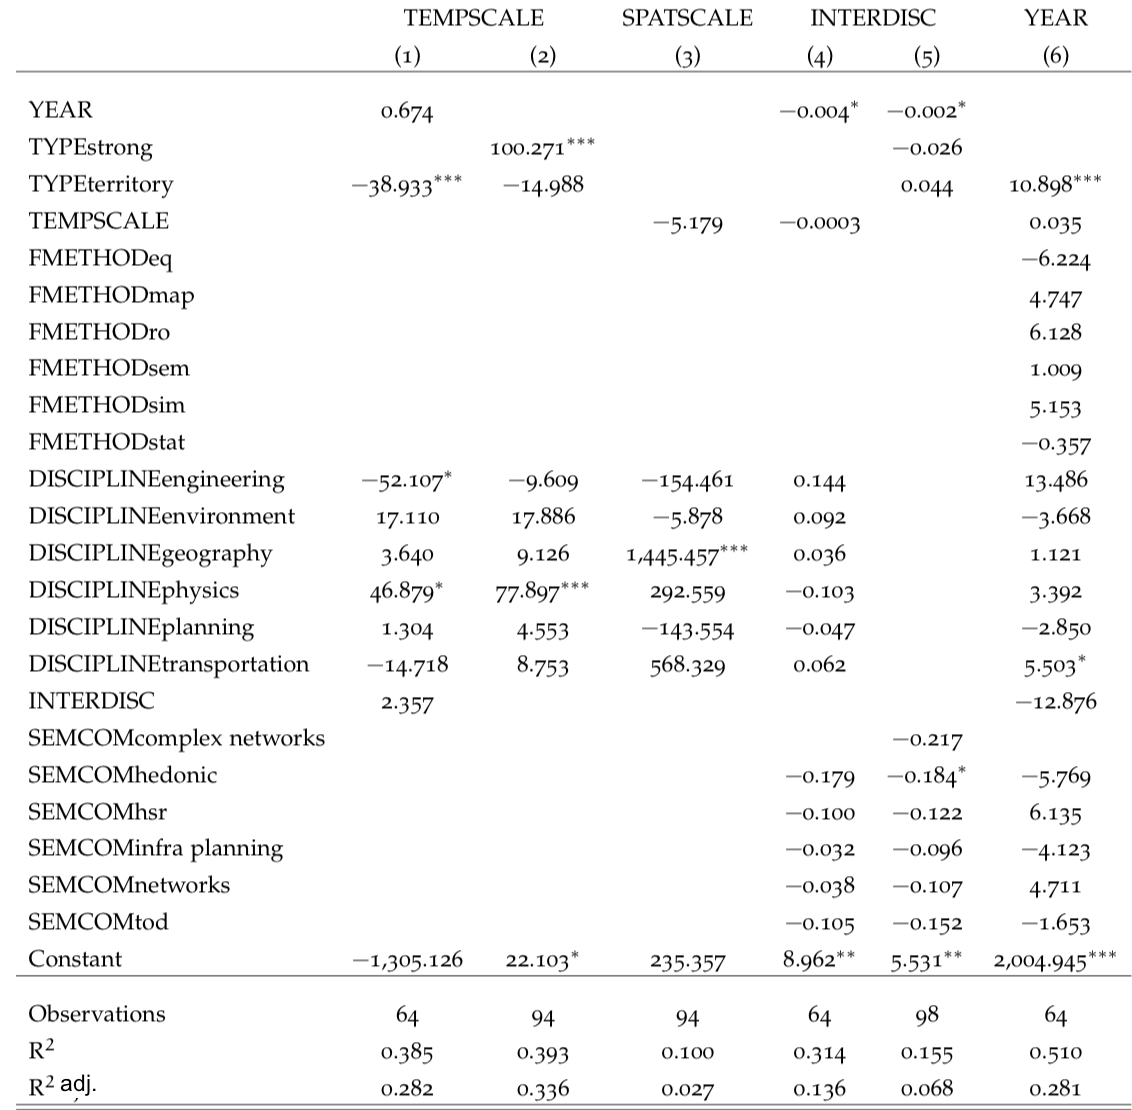
\includegraphics[height=0.92\textheight]{figures/modelography_regressions.png}


}


\sframe{Random forest regression}{

%We finally use random forest regression to compare the relative importance of variables to explain model type, and show that among different way to define disciplinary belonging, position in the citation network has the largest influence.

Random forest to classify type of model: citation class has an importance of 45\%, discipline 31\% and semantic 23\%

\bigskip

Random forest regression for interdisciplinarity: low explicative power (7.6\%); importance of variables: discipline 39\%, semantic 31\% and citation 29\%

}




\sframe{Synthesis: modeled processes}{

% synthesis : modeled processes ?
% + content of thesis models ?

\centering

\tiny
\begin{tabular}{|l|p{2.9cm}|p{2.9cm}|p{2.9cm}|}
\hline
 & Networks $\rightarrow$ Territories & Territories $\rightarrow$ Networks & Networks $\leftrightarrow$ Territories\\ \hline
\multirow{2}{*}{Micro} &
\textbf{Economics: } real estate market, relocalization, employment market & NA & \textbf{Computer Science : } spontaneous growth \\\cline{2-2}
& \textbf{Planning: } regulations, development & & \\\hline
& \textbf{Economics: } real estate market, transportation costs, amenities & \textbf{Economics: } network growth, offer and demand & \textbf{Economics: } investments, relocalizations, offer and demand, network planning\\\cline{2-4}
\multirow{2}{*}{Meso}& \textbf{Geography: } land-use, centrality, urban sprawl, network effects & \textbf{Transportation: } investments, level of governance & \textbf{Geography: } land-use, network growth, population diffusion \\\cline{2-3}
& \textbf{Planning/transportation: } accessibility, land-use, relocalization, real estate market & \textbf{Physics: } topological correlations, hierarchy, congestion, local optimization, network maintenance & \\\hline
& \textbf{Economics: } economic growth, market, land-use, agglomeration, sprawl, competition & \textbf{Economics: } interactions between cities, investments & \textbf{Economics: } offer and demand \\ \cline{2-4}
\multirow{2}{*}{Macro} & \textbf{Geography: } accessibility, interaction between cities, relocalization, political history & \textbf{Geography: } interactions between cities, potential breakdown & \textbf{Transportation: } network coverage \\\cline{2-3}
& \textbf{Transportation: } accessibility, real estate market & \textbf{Transportation: } network planing & \\\hline
\end{tabular}


}





\sframe{Discussion}{

\textbf{Developments}

\medskip

$\rightarrow$ Multiple experts corpus construction

\medskip

$\rightarrow$ Automatic extraction of features and classification

\medskip

$\rightarrow$ Automatic extraction of model modular structure, identify potential couplings

\bigskip

\textbf{Lessons for modeling}

\medskip

$\rightarrow$ multidisciplinary aspect of effectively co-evolutive models

\medskip

$\rightarrow$ importance of multiple scales and processes


}


\sframe{Epilogue I: effectively modeled processes}{

\centering

\tiny
\begin{tabular}[6pt]{|p{2.5cm}|c|p{2.5cm}|c|}
\hline
Process & Scales & Concept & Proposed models\\\hline
Preferential attachment/Gibrat  & Meso/Macro & Urban growth & Morphogenesis/Interactions \\\hline
Diffusion/Sprawl & Meso & Urban Form & Morphogenesis \\\hline
Closeness centrality/Accessibility & Meso/Macro & Accessibility & Morphogenesis/Interactions \\\hline
Direct flows & Macro & Interactions & Interactions\\\hline
Indirect flows/Tunnel effect/Betweenness centrality & Meso/Macro & Network effects & Morphogenesis/Interactions \\\hline
Network proximity & Meso & Accessibility & Morphogenesis \\\hline
Actives/employments relocations & Meso & Residential mobility & Lutecia\\\hline
Transportation governance & Meso & Governance & Lutecia\\\hline
\end{tabular}


}


\sframe{Epilogue II: models and co-evolution}{

\centering

\tiny
\begin{tabular}[6pt]{|p{3.2cm}|p{1.4cm}|p{1.4cm}|p{1.4cm}|p{1.4cm}|}
\hline
Model & Structuring effects & Individual co-evolution & Population co-evolution & Systemic co-evolution \\\hline
RBD \cite{raimbault2014hybrid} & X & X & X & NA \\\hline
Interactions \cite{raimbault2018indirect} & x & NA & NA & NA \\\hline
Weak coupling \cite{raimbault2016generation} & x & NA & NA & NA \\\hline
SimpopNet \cite{raimbault2018unveiling} & X & X & x & n.t. \\\hline
Macro co-evolution \cite{raimbault2018modeling} & X & X & X & n.t. \\\hline
Meso co-evolution \cite{raimbault2019urban} & X & X & x & NA\\\hline
Lutecia \cite{le2015modeling} & n.t. & X & n.t. & NA\\\hline
Empirical: Grand Paris \cite{raimbault2017identification} & X & x & o & NA\\\hline
Empirical: South Africa \cite{raimbault2017structural} & X & x & o & n.t.\\\hline
Empirical: France \cite{raimbault2018modeling} & o & x & o & n.t.\\\hline
\end{tabular}

}



\sframe{Conclusion}{


 % This work thus provide a systematic and broad overview on the diversity of approaches to model interaction between networks and territories, and foster the possibilities of a reflexive positioning in the context of building new models.

 % need of reflexivity : cite complexities ?

$\rightarrow$ systematic and broad overview of diverse approaches to modeling networks and territories

\medskip

$\rightarrow$ difficulty of systematic review and meta-analysis in social sciences, but new tools and methods for a reflexive positioning are crucial \cite{doi:10.1177/2399808319870816}

\medskip

$\rightarrow$ towards a quantitative, applied and reflexive epistemology


%Raimbault, J., Chasset, P.-O., Cottineau, C., Commenges, H., Pumain, D., Kosmopoulos, C., & Banos, A. (2019). Empowering open science with reflexive and spatialised indicators. Environment and Planning B: Urban Analytics and City Science. https://doi.org/10.1177/2399808319870816


\bigskip
\bigskip

\tiny
\textbf{Bibliometric tools: }

\tiny{Raimbault, J. (2019). Exploration of an interdisciplinary scientific landscape. Scientometrics, 119(2), 617-641.}

\medskip

\tiny{Raimbault, J., Chasset, P.-O., Cottineau, C., Commenges, H., Pumain, D., Kosmopoulos, C., \& Banos, A. (2019). Empowering open science with reflexive and spatialised indicators. Environment and Planning B: Urban Analytics and City Science. https://doi.org/10.1177/2399808319870816}

\medskip

Code and data available at\\
\url{https://github.com/JusteRaimbault/CityNetwork/tree/master/Models/QuantEpistemo/HyperNetwork/Modelography}




}





\sframe{Reserve slides}{

\centering

\Large

\textbf{Reserve Slides}

}


% - full stat models
% - pareto optim for model selection



\sframe{Modalities of properties}{

\tiny

\begin{itemize}
	\item Type of model (\texttt{TYPE}): strong, territory, network.
	\item Publication year (\texttt{YEAR}), integer number.
	\item Citation community (\texttt{CITCOM}), defined within the citation network: Accessibility, Geography, Infra Planning, LUTI, Networks, TOD.
	\item A priori discipline (\texttt{DISCIPLINE}): biology, computer science, economics, engineering, environment, geography, physics, planning, transportation.
	\item Semantic community (\texttt{SEMCOM}): brt, complex networks, hedonic, hsr, infra planning, networks, tod.
	\item Methodology used: ca (Cellular Automaton), eq (analytical equations), map (cartography), mas (Multi-agent simulation), ro (operations research), sem (Structural Equation Modeling), sim (simulation), stat (statistics).
	\item Interdisciplinarity index (\texttt{INTERDISC}): real number in $[0,1]$.
	\item Temporal scale (\texttt{TEMPSCALE}): given in years, is set to 0 for static analyses.
	\item Spatial scale (\texttt{SPATSCALE}): continent (10000), country (1000), region (100), metro (10). These modalities are numerically transformed in km by the values given in parenthesis (stylized scales).
\end{itemize}

}

\sframe{Linear model selection}{

\centering

% Regarding model selection, it is not achieved following a unique criteria, because of the low number of observations for some models, but by the optimization in the Pareto sense of contradictory objectives of adjustment (adjusted $R^2$, to be maximized) and of the overfitting (corrected Akaike criterion AICc, to be minimized), while controlling the number of observation points. The Fig.~\ref{fig:app:quantepistemo:regressions} gives for each variable to be explained the localization of the set of potential models within the objective space, and also the corresponding number of observations. For interdisciplinarity, two point clouds correspond to different compromises, and we select the two optimal models (one for each cloud). For the spatial scale, we postulate a positive $R^2$, and a single optimal model then emerges. For the temporal scale, we have as for interdisciplinarity two compromise models. Finally for the year, the AICc gain between the two potential optima is negligible in comparison to the $R^2$ loss, and we thus select the optimal model such that $R^2>0.25$ and AICc$<600$. The results of models are given in the following.

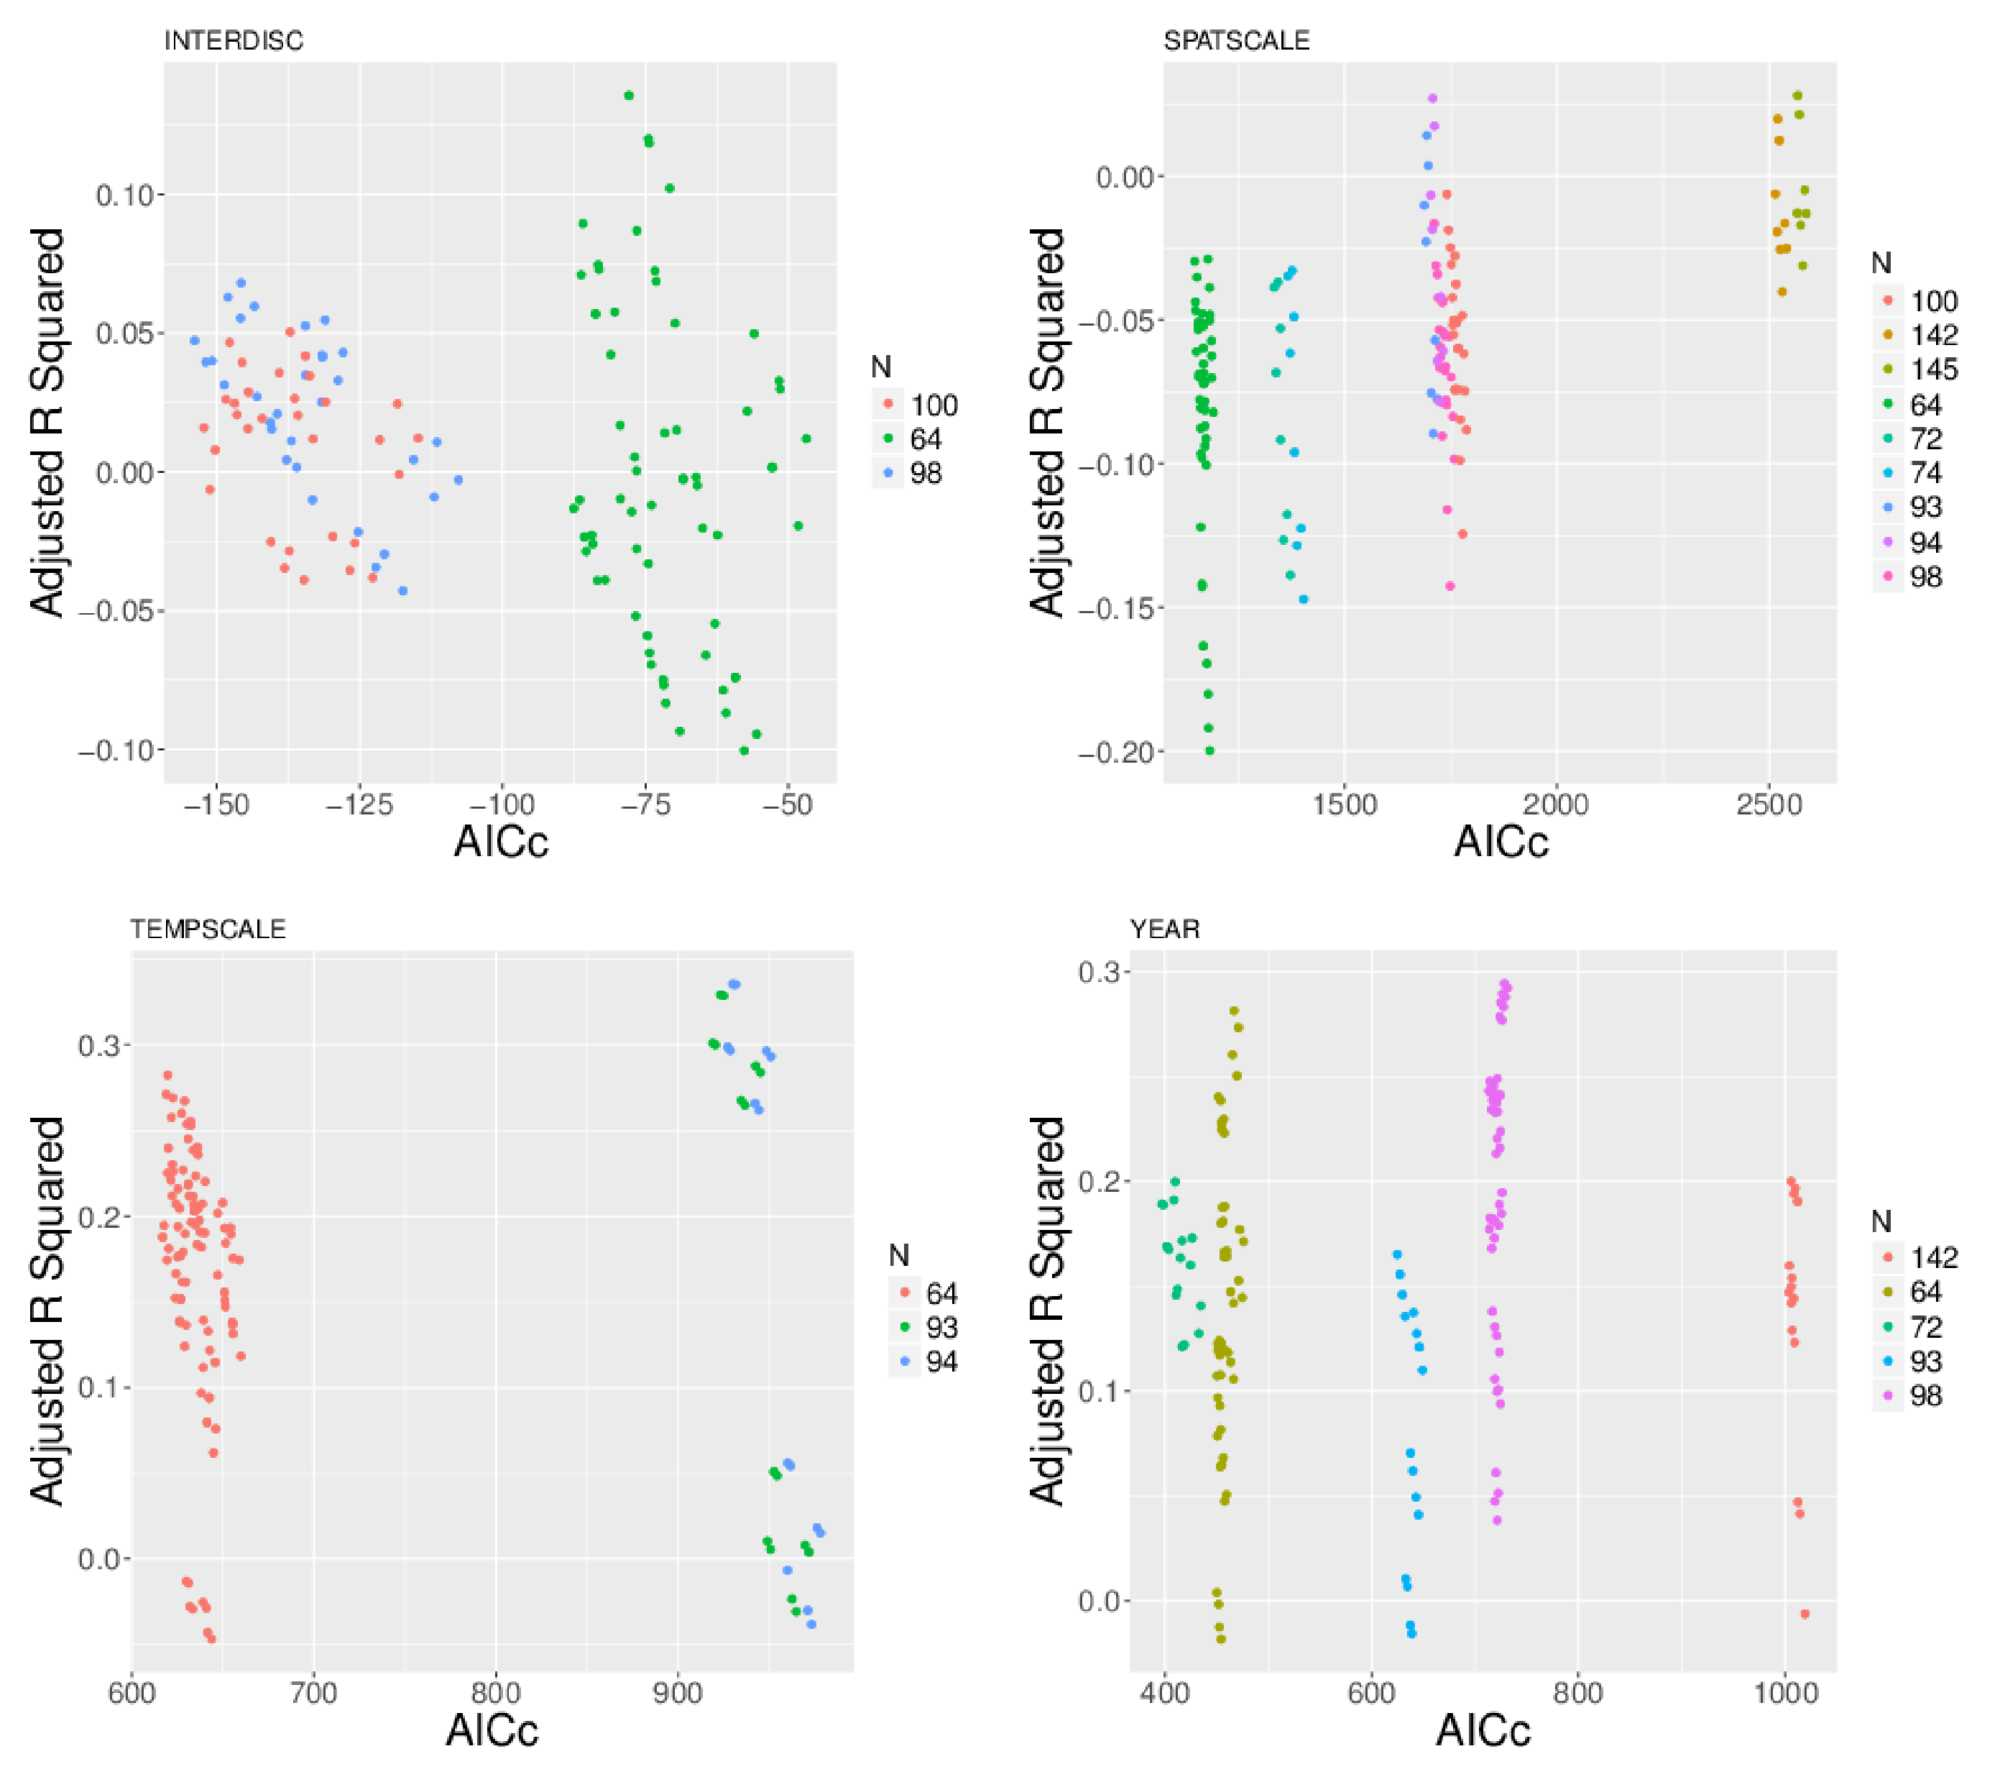
\includegraphics[height=0.9\textheight]{figures/A-quantepistemo-regressions.jpg}


}



%%%%%%%%%%%%%%%%%%%%%
\begin{frame}[allowframebreaks]
\frametitle{References}
\bibliographystyle{apalike}
\bibliography{biblio}
\end{frame}
%%%%%%%%%%%%%%%%%%%%%%%%%%%%







\end{document}




